 



\chapter{The power grid}
%\section{History of the power grid}
%conventional power Grid






\section{The Conventional Power Grid}
The \acrfull{cpg} is described in several papers, and books like \cite{BlumeStevenW2007Epsb}, as  a uni-directional, manually controlled, power distribution system.  

\begin{figure}[t]
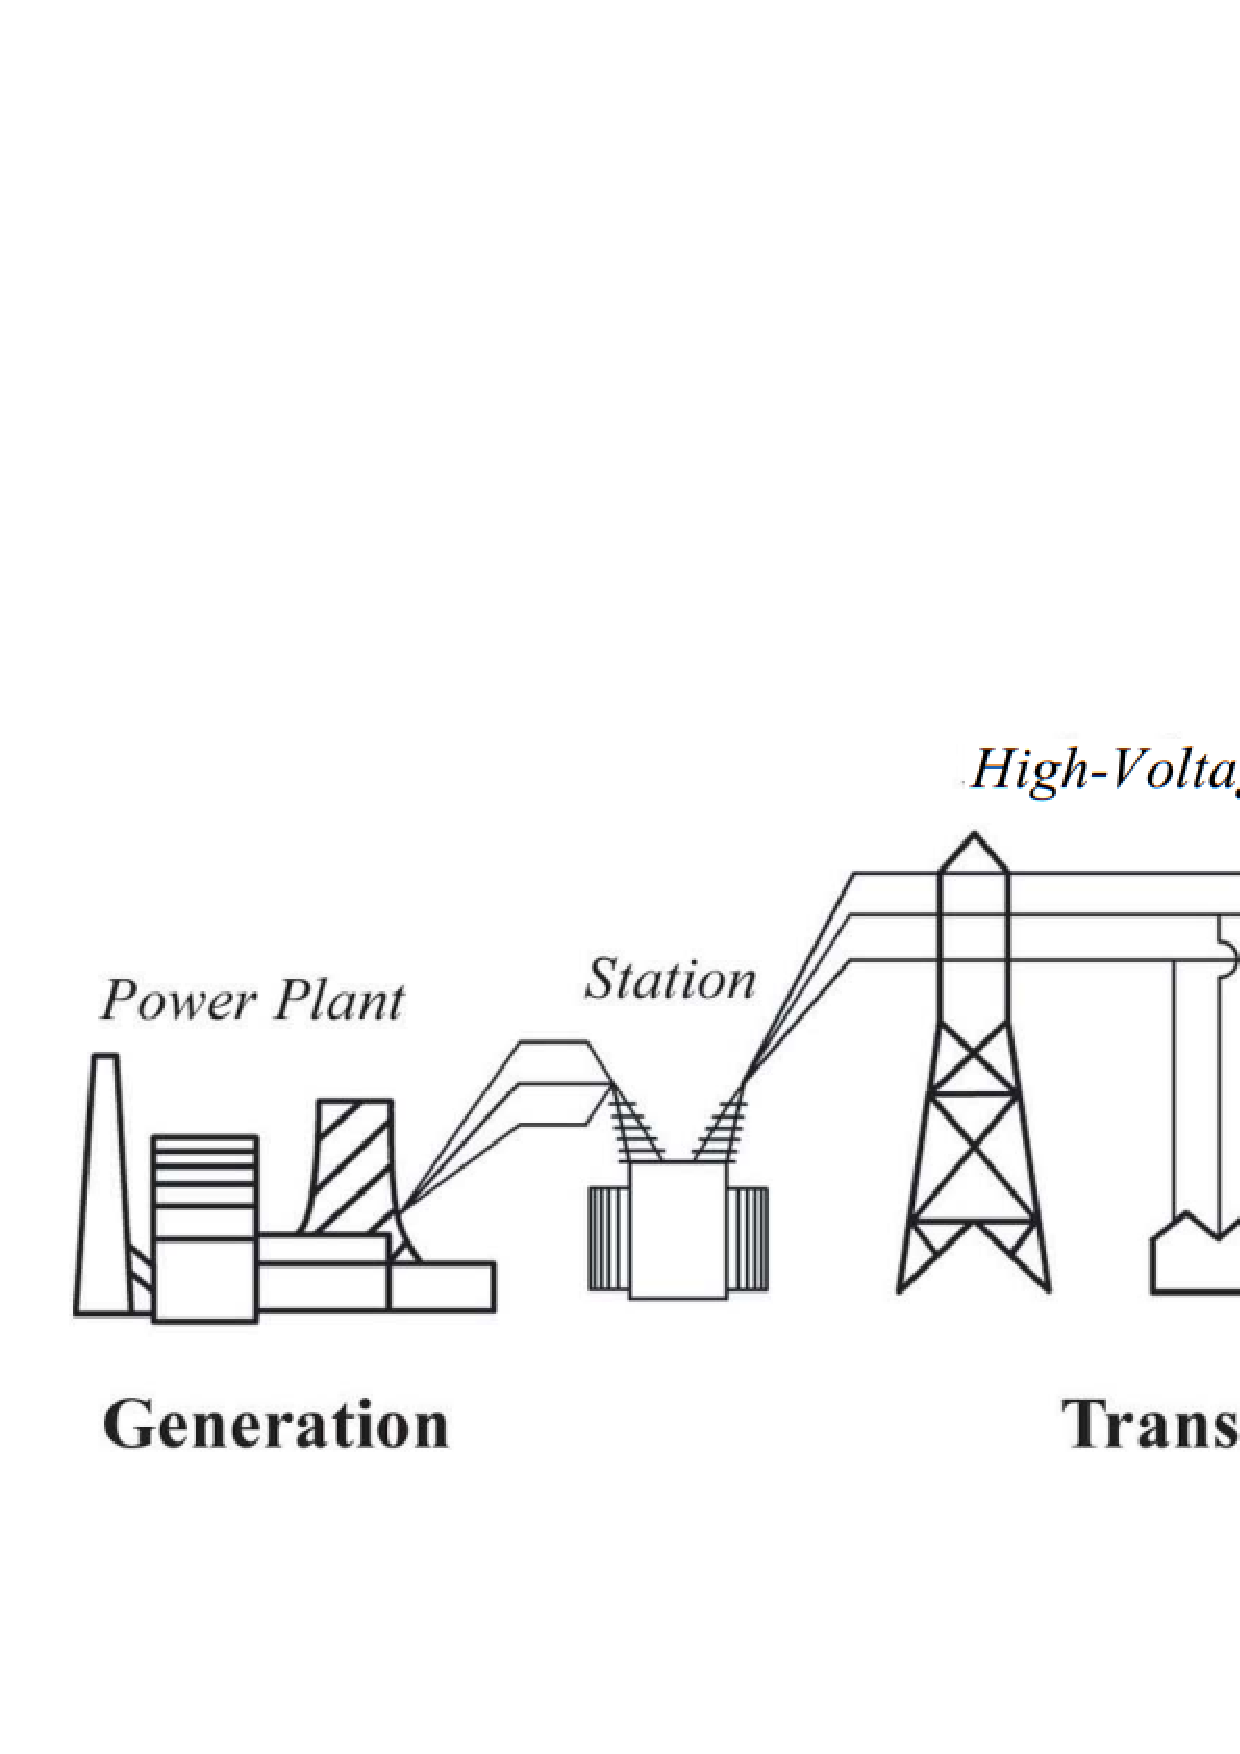
\includegraphics[width=\linewidth]{figures/Blume-PowerGrid-SystemOverView.png}
\caption[Power Grid System Overview]{Power Grid System Overview , as presented in \cite{BlumeStevenW2007Epsb}}
\label{fig:Blume-PowerGrid-SystemOverView}
\end{figure}



\subsection{Overview of the Conventional Power Grid}
The \acrlong{cpg} is a system by which electric power is centrally generated, transmitted, and distributed to industrial, residential,and commercial end users, in order to ensure a reliable access to a sufficient amount of electrical energy. 
  The \acrlong{cpg}, as described in \cite{BlumeStevenW2007Epsb}, consists of the following subsystems, visualised in figure \ref{fig:Blume-PowerGrid-SystemOverView}:

\begin{itemize}

 \item The \textbf{Generation Subsystem} which Generates electric power from various sources of energy, to be transmitted for distribution to Consumers. Some examples of installations generating electrical power are nuclear power plants, as well as hydroelectric power plants, feeding water-driven turbines in order to generate power.
 \item The \textbf{Transmission Subsystem} which transmits electric power from the Generation subsystem to the Distribution Subsystem. The current is transmitted via high voltage power lines, minimising energy loss over longer distances.
 \item The \textbf{Distribution Subsystem} which distributes electric power to end users, after converting the high voltage input into lower voltage levels, suitable for consumption.
 \end{itemize}


\subsection{Characteristics of the Conventional Power Grid} \label{subsec:PG-char}


In order to provide a description of the \acrfull{sg}, a description of the characteristics of the \acrlong{cpg} is provided.

As described in  \cite{BlumeStevenW2007Epsb} by \citeauthor{BlumeStevenW2007Epsb}, some of the characteristics of the \acrlong{cpg} are:

\begin{itemize}
\item Power is generated in real time. In the event a consumer is "flipping a power switch," the power grid must have sufficient resources in order to keep the voltage levels at an acceptable level.
\item The \acrlong{cpg} is controlled by a central management facility known as the \acrfull{scada} subsystem. The monitoring and management of the \acrshort{pg} is initiated from the Control Center, utilising unidirectional communication channels. 
\item The \acrlong{cpg} \acrlong{scada} subsystem is offline, i. e. not connected to any publicly available computer network, and thus unavailable from the Internet. Therefore, operational duties must be performed by authorised personnel physically located\footnote{External personnel must physically travel to the site, to perform maintenance tasks, for instance.} at designated operational sites.

\end{itemize}

The \acrlong{cpg} originates from the local society-serving power generation facilities initiating the supply of electrical power, which over the years were interconnected to form a grid, connecting consumers to a network of several power generating facilities, providing a more flexible power distribution infrastructure. 
As described in Chapter 2.3 of \cite{Rihan2018} %\cite{SmartGridOverview2013}
, the \acrlong{cpg} is facing challenges, related to Black Outs adhering to the increased demands for electrical power. 


%\section{The Smart Grid}
%smart Grid
\section{The Smart Grid}
\subsection{Overview of The Smart Grid}

The \acrfull{sg} is, as described by \citeauthor{humayed2017cyber} in \cite{humayed2017cyber}, the modernisation of the \acrfull{cpg}, into what may be described as an exapmle of a \acrfull{cps}.


\begin{figure}[t]
\includegraphics[width=\linewidth]{figures/NIST-SmartGRID-ConceptualModel.png}
\caption[Smart Grid Conceptual Model]{Updated \acrlong{sg} conceptual model, as presented in \cite[p. 13]{gopstein2021nist}, Figure 4}
\label{fig:NIST-SmartGRID-ConceptualModel}
\end{figure}

\subsubsection{Cyber-Physical System}

As described by \citeauthor{humayed2017cyber} in \cite{humayed2017cyber}, a \acrfull{cps} is characterised by using a computer-based system in order to control and monitor systems of the physical world. The \acrshort{cps} is utilised in order to control physical systems from various fields of applications. Humayed et. al., in \cite{humayed2017cyber}, describes as various appliances as \acrfull{ics}, Medical Devices, and \acrlong{sg}.
The Smart Grid, therefore, is an example of a \acrfull{cps}, consisting of the physical system of a Power Grid, under the control of a network/Cyberspace-connected system. 

Due to the shortcomings of the \acrshort{cpg} previously\footnote{Refer to subsection \ref{subsec:PG-char}, and Chapter 2.3 of [7]} covered, the \acrshort{sg} might be described as an effort to reduce the risk of blackouts, and to generally make the power distribution system more robust and reliable, meeting the increasing demand for electrical power.
 
\begin{table}[t]
    \centering
 
    \begin{tabular}{|p{0.3cm}|p{2.2cm}|p{9.1cm}|}
   \hline

 &\textbf{Domain} & \textbf{Roles/Services in the Domain} \\ \hline
 
1 & \textbf{Customer} & The end users of electricity. May also generate, store, and manage the use of energy. Traditionally, three customer types are discussed, each with its own sub-domain: residential, commercial, and industrial. \\ \hline
2 & \textbf{Markets} & The facilitators and participants in electricity markets and other economic mechanisms used to drive action and optimize system outcomes. \\ \hline
3 & \textbf{Service Provider} & The organizations providing services to electrical customers and to utilities. \\ \hline
4 & \textbf{Operations} & The managers of the movement of electricity. \\ \hline
5 & \textbf{Generation Including DER} & The producers of electricity. May also store energy for later distribution. This domain includes traditional generation sources and distributed energy resources (DER). At a logical level, “generation” includes those traditional larger scale technologies usually attached to the transmission system, such as conventional thermal generation, large-scale hydro generation, and utility-scale renewable installations usually attached to transmission. DER is associated with generation, storage, and demand response provided in the customer and distribution domains, and with service provider-aggregated energy resources. \\ \hline
6 & \textbf{Transmission} & The carriers of high voltage electricity over long distances. May also store and generate electricity. \\ \hline
7 & \textbf{Distribution} & The distributors of electricity to and from customers. May also store and generate electricity.\\
    \hline


    
    \end{tabular}

    \caption[Domains and roles/services in the smart grid conceptual model]{Domains and roles/services in the smart grid conceptual model, as presented in Table 1 of \cite{gopstein2021nist}}
    \label{tab:nist-domains}
\end{table}


\section{Smart Grid models}
In order to improve the understanding of a vastly complex system like the \acrlong{sg}, some organisations, like the \acrfull{nist}, as well as the \acrfull{eu} commission for \acrshort{sg}, is maintaining theoretical models. I have chosen to present a brief overview of the \acrshort{nist} model in order to provide a brief overview of various parts of the \acrlong{sg}, and thereafter focus on the \acrlong{wams} and related concepts.

%In order to provide a broader overview of the concept of the \acrlong{sg}, I choose to present two models the \acrshort{nist} conceptual model, as well as the \acrshort{eu} \acrlong{sgam}.


\subsection{The NIST Conceptual model}



In order to improve the understanding of a vastly complex system like the \acrlong{sg},
the \acrfull{nist} is maintaining the Conceptual model of the \acrlong{sg}. The graphical visualisation of the model, as presented in \cite[p. 13]{gopstein2021nist}, Figure 4,  is  shown in 
Figure \ref{fig:NIST-SmartGRID-ConceptualModel}.
The \acrlong{sg} adds Information and Communication Technology (ICT) to the \acrlong{cpg}, in order to transform the  unidirectional communication lines of the monitoring and control infrastructure of the \acrlong{cpg}, into an infrastructure utilising two-way communication between the various parts of the \acrlong{sg} infrastructure. 
%\subsection{The Smart Grid: Critical Information Infrastructure}
%According to \cite[p. 610]{Bîrleanu2019}, the \acrlong{sg} consists of the following subsystems:

%\begin{itemize}
%\item \textbf{the conventional  power grid}
%\item \textbf{intelligent equipment} 
%\item \textbf{communication infrastructure}
%\end{itemize}

%\cite{Bompard2012}...

%...\acrlong{sg} Subsystems
%\begin{itemize}
%\item 
%\end{itemize}

\subsubsection{The Smart Grid Domains}

Table \ref{tab:nist-domains} gives an overview of the roles and services of the \acrshort{sg} domain as presented by \acrshort{nist} in \cite{gopstein2021nist}.\\  

The \acrlong{sg} is a complex system, involving many aspects like, for instance applications, various kinds of layers and relations between domains, to name a few, topics which it will be beyond the scope of this thesis to cover. My thesis will focus on various aspects of the \acrshort{sg} \acrlong{wams} for the remaining part of the thesis.










